% \documentclass[dvipdfmx, 11pt]{beamer}
\documentclass[aspectratio=169, dvipdfmx, 11pt]{beamer}

\usepackage{here, amsmath, latexsym, amssymb, bm, ascmac, mathtools, multicol, tikz}
\usetikzlibrary{shapes,arrows,positioning,automata,decorations.pathmorphing,patterns}

%デザインの選択
\usetheme{Luebeck}
\usecolortheme{orchid}
\usefonttheme{professionalfonts}
\useinnertheme{circles}
\useoutertheme{infolines}

%しおりの文字化け解消
\usepackage{atbegshi}
\usepackage{pxjahyper}

%ナビゲーションバー非表示
\setbeamertemplate{navigation symbols}{}
%既定をゴシック体に
\renewcommand{\kanjifamilydefault}{\gtdefault}
%タイトル・フレームタイトル色
\setbeamercolor{title}{fg=structure, bg=}
\setbeamercolor{frametitle}{fg=structure, bg=}
%itemize
\setbeamertemplate{itemize item}{\small\raise0.5pt\hbox{$\bullet$}}
\setbeamertemplate{itemize subitem}{\tiny\raise1.5pt\hbox{$\blacktriangleright$}}

% color
\newcommand{\red}[1]{\textcolor{red}{#1}}
\newcommand{\green}[1]{\textcolor{green!40!black}{#1}}
\newcommand{\blue}[1]{\textcolor{blue!80!black}{#1}}

\title[論文紹介]{論文紹介}
\subtitle{Distributional Reinforcement Learning\\with Quantile Regression\\{\small (分位回帰による分布的強化学習)}}
\author{【氏名】}
\institute{【研究室名】 \quad 指導教員：【指導教員名】}
\date{2026/07/12}

\begin{document}

\maketitle

\begin{frame}{目次}
  \tableofcontents
\end{frame}

%%%%%%%%%%%%%%%%%%%%%%%%%%%%%%%%%%%%%%%%%%%%%%%%%%%%%
% 論文情報
%%%%%%%%%%%%%%%%%%%%%%%%%%%%%%%%%%%%%%%%%%%%%%%%%%%%%
\begin{frame}{紹介する論文について}
  \begin{itemize}
    \item \textbf{タイトル}: Distributional Reinforcement Learning with Quantile Regression
    \item \textbf{著者}: Will Dabney, Mark Rowland, Marc G.\ Bellemare, Rémi Munos（DeepMind）
    \item \textbf{会議等}: AAAI 2018 (arXiv:1710.10044)
  \end{itemize}
  \vfill
  \begin{block}{一言でいうと}
    先行研究C51ではValue distributionを\textbf{固定位置の離散分布}で近似しKLダイバージェンスで学習していたが、
    本論文では\textbf{固定確率・可変位置}の\alert{分位分布}（quantile distribution）で近似し、
    \alert{分位回帰}によりWasserstein距離を直接最小化する手法（QR-DQN）を提案した。
    理論と実践のギャップを埋め、Atariゲームで当時のSOTAを大幅に更新した。
  \end{block}
\end{frame}

%%%%%%%%%%%%%%%%%%%%%%%%%%%%%%%%%%%%%%%%%%%%%%%%%%%%%
% 背景知識の復習
%%%%%%%%%%%%%%%%%%%%%%%%%%%%%%%%%%%%%%%%%%%%%%%%%%%%%
\section{背景知識の復習}

\begin{frame}{復習：Distributional RL}
  \begin{block}{前回のおさらい：Value Distribution}
    従来のRLは累積報酬の期待値$Q^\pi(x,a)$のみを学習するが、
    Distributional RLでは累積報酬の\alert{分布全体}を学習する。
  \end{block}
  \vfill
  \begin{itemize}
    \item \textbf{確率変数} $Z^\pi(x,a) = \sum_{t=0}^{\infty} \gamma^t R_t$：累積報酬そのもの
    \begin{itemize}
      \item $R_t$：時刻$t$の報酬、$\gamma \in [0,1)$：割引率
    \end{itemize}
    \item $Q^\pi(x,a) = \mathbb{E}[Z^\pi(x,a)]$ は単にその\textbf{期待値}
    \item \textbf{分布的Bellman方程式}：$Z^\pi(x,a) \overset{D}{=} R(x,a) + \gamma Z^\pi(X', A')$
    \begin{itemize}
      \item $X' \sim P(\cdot|x,a)$：次状態、$A' \sim \pi(\cdot|X')$：次行動
      \item $\overset{D}{=}$は「分布として等しい」の意味
    \end{itemize}
  \end{itemize}
  \vfill
  {\small 分布を学ぶことで、まれだが重要なイベントの情報を保持でき、学習が安定する。}
\end{frame}

%%%%%%%%%%%%%%%%%%%%%%%%%%%%%%%%%%%%%%%%%%%%%%%%%%%%%
% C51の復習と課題
%%%%%%%%%%%%%%%%%%%%%%%%%%%%%%%%%%%%%%%%%%%%%%%%%%%%%
\begin{frame}{復習：C51アルゴリズムとその課題}
  \begin{block}{C51の手法（Bellemare et al., 2017）}
    Value distributionを\textbf{$N$個の固定位置}（アトム）$z_1 \leq \cdots \leq z_N$上の離散分布で近似。
    ネットワークは各アトムの\textbf{確率}$q_i$を出力する。
    \vspace{-4pt}
    \[
      z_i = V_{\min} + i \cdot \Delta z, \quad \Delta z = \frac{V_{\max} - V_{\min}}{N-1}
    \]
    \vspace{-8pt}
    {\small 学習は射影$\Phi$を行った上で\textbf{KLダイバージェンス}を最小化。}
  \end{block}
  \vfill
  \begin{alertblock}{C51の課題（本論文のモチベーション）}
    \begin{enumerate}
      \item 台の範囲$[V_{\min}, V_{\max}]$を\red{事前に固定}する必要がある
      \item Bellman更新で台がずれるため\red{射影ステップ}が必要
      \item KLダイバージェンスを最小化 → 理論的に保証されたWasserstein距離との\red{乖離}
    \end{enumerate}
  \end{alertblock}
  \vfill
  {\small → 分布的Bellman作用素$\mathcal{T}^\pi$はWasserstein距離で縮小写像だが、C51はそれを活用できていない。}
\end{frame}

%%%%%%%%%%%%%%%%%%%%%%%%%%%%%%%%%%%%%%%%%%%%%%%%%%%%%
% Wasserstein距離
%%%%%%%%%%%%%%%%%%%%%%%%%%%%%%%%%%%%%%%%%%%%%%%%%%%%%
\section{理論的基盤}

\begin{frame}{Wasserstein距離と逆CDF}
  \begin{block}{$p$-Wasserstein距離（論文Section 2）}
    {\small 2つの分布$Y, U$の$p$-Wasserstein距離は逆CDFの$L^p$距離で表せる}
    {\small
    \[
      W_p(Y, U) = \left(\int_0^1 \left|F_Y^{-1}(\omega) - F_U^{-1}(\omega)\right|^p \, d\omega \right)^{1/p}
    \]
    }
    {\scriptsize $F_Y^{-1}(\omega) = \inf\{z \in \mathbb{R} : F_Y(z) \geq \omega\}$：$Y$の逆CDF（分位関数）。$\omega \in [0,1]$：積分変数。}\\
    {\scriptsize $p = \infty$の場合：$W_\infty(Y, U) = \sup_{\omega \in [0,1]} |F_Y^{-1}(\omega) - F_U^{-1}(\omega)|$。}
  \end{block}
  \vfill
  \begin{exampleblock}{分布的Bellman作用素の縮小写像性（Lemma 1, Bellemare et al., 2017）}
    {\small 最大化Wasserstein距離$\bar{d}_p(Z_1, Z_2) = \sup_{x,a} W_p(Z_1(x,a), Z_2(x,a))$のもとで}
    {\small
    \[
      \bar{d}_p(\mathcal{T}^\pi Z_1, \mathcal{T}^\pi Z_2) \leq \gamma \cdot \bar{d}_p(Z_1, Z_2)
    \]
    }
    {\scriptsize → $\mathcal{T}^\pi$の繰り返し適用で$Z^\pi$に収束。}
  \end{exampleblock}
\end{frame}

%%%%%%%%%%%%%%%%%%%%%%%%%%%%%%%%%%%%%%%%%%%%%%%%%%%%%
% Wasserstein距離の直接最小化におけるバイアスの問題
%%%%%%%%%%%%%%%%%%%%%%%%%%%%%%%%%%%%%%%%%%%%%%%%%%%%%
\begin{frame}{Wasserstein距離の直接最小化におけるバイアスの問題}
  \begin{alertblock}{Theorem 1（Bellemare et al., 2017）：バイアスの存在}
    {\small
    真の分布$B$からのサンプルの経験分布$\hat{Y}_m$を用いて、
    モデル分布$B_\mu$を確率的に最適化しようとすると、一般に\red{バイアス}が生じる
    \vspace{-4pt}
    \[
      \operatorname*{arg\,min}_\mu \mathbb{E}\!\left[W_p(\hat{Y}_m, B_\mu)\right]
      \neq \operatorname*{arg\,min}_\mu W_p(B, B_\mu)
    \]
    \vspace{-4pt}
    }
  \end{alertblock}
  \begin{itemize}\setlength{\itemsep}{2pt}
    \item {\small $B$: 近似したい真の分布、$B_\mu$: パラメータ$\mu$で特徴づけられるモデル分布}
    \item {\small $\hat{Y}_m$: 分布$B$からの$m$個のサンプルの経験分布}
    \item {\small \textbf{期待値と分布}：\\
      右辺の真の分布$B$は、経験分布$\hat{Y}_m$の期待値（平均的な分布）として $B = \mathbb{E}[\hat{Y}_m]$ と書ける。\\
      ※ここで期待値$\mathbb{E}$をとっているが、スカラー値ではなく\textbf{確率分布}になることに注意。}
  \end{itemize}
\end{frame}

\begin{frame}{具体例を用いた直感的な理解（コイントス） 1/2}
  \begin{block}{コイントス（ベルヌーイ分布）の例}
    {\small
    真の分布$B$を「確率 $p=0.4$ で1、$0.6$ で0が出るコイン」とし、モデル$B_\mu$（確率$\mu$で1）で近似する。
    \begin{itemize}\setlength{\itemsep}{3pt}
      \item \textbf{真の目標（右辺）}: $W_1(B, B_\mu) = |0.4 - \mu|$ を最小化するため、最適解は \textbf{$\mu = 0.4$}。
      \item \textbf{確率的勾配法による最適化（左辺）}:
      初期値 \textbf{$\mu_0 = 0.5$} とし、毎ステップ3回引き目標値 $S/3$ ($S$は1の回数) に向けて更新する。
      $S$ の値（目標値）による更新方向の場合分けは以下のようになる。
      \begin{itemize}\setlength{\itemsep}{2pt}
        \item \textbf{$S \le 1$（目標値 $0$ または $\approx 0.33$）の場合}:\\
        現在の $\mu=0.5$ よりも目標値が小さいため、$\mu$ は\textbf{減少方向}へ更新。
        \item \textbf{$S \ge 2$（目標値 $\approx 0.67$ または $1$）の場合}:\\
        現在の $\mu=0.5$ よりも目標値が大きいため、$\mu$ は\textbf{増加方向}へ更新。
      \end{itemize}
    \end{itemize}
    }
  \end{block}
\end{frame}

\begin{frame}{具体例を用いた直感的な理解（コイントス） 2/2}
  \begin{block}{なぜバイアスが生じるのか？}
    {\small
    \begin{itemize}\setlength{\itemsep}{4pt}
      \item $S \sim \text{Binomial}(3, 0.4)$ で各 $S$ が出る確率を計算すると、
      \begin{itemize}\setlength{\itemsep}{2pt}
        \item $P(S=0) = 0.6^3 = 0.216$
        \item $P(S=1) = 3 \times 0.4 \times 0.6^2 = 0.432$ \quad $\to P(S \le 1) = \alert{0.648}$
        \item $P(S=2) = 3 \times 0.4^2 \times 0.6 = 0.288$ \quad $\to P(S \ge 2) = 0.352$
        \item $P(S=3) = 0.4^3 = 0.064$
      \end{itemize}
      \item 減少する確率 ($0.648$) が増加する確率 ($0.352$) より高いため、$\mu$ は $0.5$ から減少する可能性が高い。
      \item 減少確率と増加確率が均衡 ($0.5$) するのは、累積確率が $0.5$ に達する $S/3$ の\textbf{中央値（メディアン）}、すなわち \alert{$\mu \approx 0.33$} の地点である。
      \item $\to$ 確率的勾配法では $0.33$ に収束し、真の最適解 $0.4$ と\alert{一致しない}（バイアス）。
    \end{itemize}
    }
  \end{block}
\end{frame}

\begin{frame}{本論文の問い}
  \begin{exampleblock}{分位回帰によるバイアスの解消}
    Wasserstein距離の縮小写像性を活用しつつ、\alert{バイアスのない}方法で学習できるアルゴリズムは存在するか？\\
    → \alert{分位回帰}（quantile regression）により実現できる！
  \end{exampleblock}
\end{frame}

%%%%%%%%%%%%%%%%%%%%%%%%%%%%%%%%%%%%%%%%%%%%%%%%%%%%%
% 分位分布の導入
%%%%%%%%%%%%%%%%%%%%%%%%%%%%%%%%%%%%%%%%%%%%%%%%%%%%%
\section{提案手法：分位分布と分位回帰}

\begin{frame}{C51から分位分布への「転置」}
  \begin{columns}[T]
    \begin{column}{0.48\textwidth}
      \begin{block}{C51（固定位置・可変確率）}
        {\small
        $N$個の\textbf{固定}された位置$z_1, \dots, z_N$に対し、
        各位置の\textbf{確率}$q_1, \dots, q_N$をパラメータとする
        \[
          Z(x,a) = \sum_{i=1}^{N} q_i \, \delta_{z_i}
        \]
        }
      \end{block}
    \end{column}
    \begin{column}{0.48\textwidth}
      \begin{exampleblock}{QR-DQN（固定確率・可変位置）}
        {\small
        $N$個の\textbf{均等}な確率$\frac{1}{N}$に対し、
        各位置$\theta_1, \dots, \theta_N$を\alert{パラメータ}とする
        \[
          Z_\theta(x,a) = \frac{1}{N}\sum_{i=1}^{N} \delta_{\theta_i(x,a)}
        \]
        }
      \end{exampleblock}
    \end{column}
  \end{columns}
  \vfill
  {\small $\delta_z$：$z \in \mathbb{R}$に置かれたDirac測度。}\\[4pt]
  \textbf{分位分布の利点}：
  \begin{enumerate}
    \item 台の範囲$[V_{\min}, V_{\max}]$の\blue{事前設定が不要}（位置が自由に動くため）
    \item 射影ステップが\blue{不要}（台のずれの問題が起きない）
    \item \alert{分位回帰}により、バイアスのない勾配でWasserstein距離を最小化可能
  \end{enumerate}
\end{frame}

%%%%%%%%%%%%%%%%%%%%%%%%%%%%%%%%%%%%%%%%%%%%%%%%%%%%%
% 分位射影
%%%%%%%%%%%%%%%%%%%%%%%%%%%%%%%%%%%%%%%%%%%%%%%%%%%%%
\begin{frame}{1-Wasserstein距離の最小化と分位射影}
  \begin{columns}[T]
    \begin{column}{0.62\textwidth}
      分布$Y$を分位分布$Z_\theta$で最もよく近似する位置$\theta_i$はどこか？
      \begin{block}{Lemma 2：最適な分位位置}
        {\footnotesize CDFが$F$の分布に対し、$\tau < \tau'$の区間$[\tau, \tau']$で1-Wasserstein距離
        $\int_{\tau}^{\tau'} |F^{-1}(\omega) - \theta|\,d\omega$ を最小化する$\theta$は
        \vspace{-0.6em}
        \[
          \theta^* = F^{-1}\!\left(\frac{\tau + \tau'}{2}\right)
        \]
        \vspace{-0.8em}
        }
        
        {\scriptsize $F^{-1}$が$(\tau+\tau')/2$で連続なら$\theta^*$は一意。}
      \end{block}
      \vspace{-0.2em}
      {\footnotesize
      累積確率を$\tau_i = \frac{i}{N}$（$i = 0, \dots, N$）とすると、\textbf{分位中点}は
      \vspace{-0.6em}
      \[
        \hat{\tau}_i = \frac{\tau_{i-1} + \tau_i}{2} = \frac{2i - 1}{2N}, \; i = 1, \dots, N
      \]
      \vspace{-0.6em}
      }
    \end{column}
    \begin{column}{0.36\textwidth}
      \begin{center}
      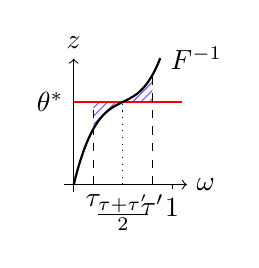
\begin{tikzpicture}[x=2.5cm, y=1cm, scale=0.5]
        \draw[->] (-0.1, 0) -- (1.15, 0) node[right] {$\omega$};
        \draw[->] (0, -0.2) -- (0, 3.2) node[above] {$z$};
        
        \draw (1, 0) -- (1, -0.1) node[below] {$1$};
        
        \fill[pattern=north east lines, pattern color=blue!60]
          (0.2, 2.1) -- plot[domain=0.2:0.5, samples=20] (\x, {12*(\x-0.5)^3 + 1.2*(\x-0.5) + 2.1}) -- (0.5, 2.1) -- cycle;
        \fill[pattern=north east lines, pattern color=blue!60]
          (0.5, 2.1) -- plot[domain=0.5:0.8, samples=20] (\x, {12*(\x-0.5)^3 + 1.2*(\x-0.5) + 2.1}) -- (0.8, 2.1) -- cycle;
          
        \draw[thick, red] (0, 2.1) node[left, black] {$\theta^*$} -- (1.1, 2.1);
        \draw[thick, domain=0:0.88, samples=40] plot (\x, {12*(\x-0.5)^3 + 1.2*(\x-0.5) + 2.1}) node[right] {$F^{-1}$};
        
        \draw[dashed] (0.2, 0) node[below] {$\tau$} -- (0.2, 2.1);
        \draw[dashed] (0.8, 0) node[below] {$\tau'$} -- (0.8, 2.784);
        \draw[dotted] (0.5, 0) node[below] {$\frac{\tau+\tau'}{2}$} -- (0.5, 2.1);
      \end{tikzpicture}
      \end{center}
    \end{column}
  \end{columns}
  \vspace{-1.0em}
  {\footnotesize
  最適な位置は$\theta_i = F_Y^{-1}(\hat{\tau}_i)$、すなわち$Y$の$\hat{\tau}_i$-分位点。\\
  元の分布$Y$を、累積確率$\tau_i$とその分位点$\theta_i$を用いて$N$個の要素を持つ離散分布$Z$に変換するこの射影操作を$\Pi_{W_1}$と書き、$\Pi_{W_1}Z$は$Z$への1-Wasserstein射影を表す。
  }
\end{frame}

%%%%%%%%%%%%%%%%%%%%%%%%%%%%%%%%%%%%%%%%%%%%%%%%%%%%%
% 分位回帰
%%%%%%%%%%%%%%%%%%%%%%%%%%%%%%%%%%%%%%%%%%%%%%%%%%%%%
\begin{frame}{分位回帰（Quantile Regression）}
  {\small 分位点をサンプルから推定する統計的手法。今回はこれを適用する。}
  \begin{block}{分位回帰損失（論文Eq.~8）}
    {\small 分位$\tau \in [0,1]$に対する分位回帰損失：}
    {\small
    \vspace{-6pt}
    \[
      \rho_\tau(u) = u \cdot (\tau - \mathbb{I}\{u < 0\}), \quad u \in \mathbb{R}
    \]
    \vspace{-8pt}
    }
    {\scriptsize $\mathbb{I}\{\cdot\}$：指示関数。過大評価を重み$\tau$で、過小評価を重み$1-\tau$で非対称にペナルティ。}
  \end{block}
  {\small 分位分布の最適位置$\theta_1, \dots, \theta_N$は、サンプル$z$を用いて以下の目的関数を最小化する}
  {\small
  \vspace{-6pt}
  \[
    \sum_{i=1}^{N} \mathbb{E}_{z \sim Z}\!\left[\rho_{\hat{\tau}_i}(z - \theta_i)\right]
  \]
  \vspace{-8pt}
  }
  {\scriptsize → ニューラルネットの出力$\theta_1, \dots, \theta_N$を同時に最適化する損失関数として使える。}
\end{frame}

%%%%%%%%%%%%%%%%%%%%%%%%%%%%%%%%%%%%%%%%%%%%%%%%%%%%%
% サンプルによる最適化が真の分位点に収束する
%%%%%%%%%%%%%%%%%%%%%%%%%%%%%%%%%%%%%%%%%%%%%%%%%%%%%
\begin{frame}{サンプルによる最適化が真の分位点に収束する}
  \begin{exampleblock}{p.7 の不等式（Theorem 1）との対比}
    {\small p.7 では $\operatorname*{arg\,min}_\mu \mathbb{E}[W_p(\hat{Y}_m, B_\mu)] \;\red{\neq}\; \operatorname*{arg\,min}_\mu W_p(B, B_\mu)$ であった。\\
    分位回帰損失では、サンプル$z$を用いた確率的勾配法でも\green{等号が成立}する。
    \vspace{-6pt}
    \[
      \operatorname*{arg\,min}_\theta \mathbb{E}_{z \sim Z}[\rho_\tau(z - \theta)]
      \;\green{=}\; F_Z^{-1}(\tau) \quad \text{（真の分位点）}
    \]
    \vspace{-8pt}
    }
  \end{exampleblock}
  \begin{block}{なぜこの等式が成り立つのか？}
    {\small
    $\rho_\tau(z - \theta)$ を $\theta$ で微分すると、勾配は $\mathbb{I}\{z < \theta\} - \tau$ となる。
    この勾配の真の分布 $Z$ に対する\textbf{期待値}をとると、
    $\mathbb{E}_Z [ \mathbb{I}\{Z < \theta\} - \tau ] = P(Z < \theta) - \tau$\\
    勾配の期待値がゼロ（＝収束点）は $\alert{P(Z < \theta) = \tau}$、すなわち
    \textbf{「累積確率が $\tau$ になる点」= 分位点の定義}そのもの！\\[2pt]
    → 勾配が\green{$\theta$に対して線形}であるため、Wasserstein距離のように\\
    \hspace{1em}期待値と非線形関数が干渉してバイアスを生むことがない。
    }
  \end{block}
\end{frame}

%%%%%%%%%%%%%%%%%%%%%%%%%%%%%%%%%%%%%%%%%%%%%%%%%%%%%
% Huber分位回帰損失
%%%%%%%%%%%%%%%%%%%%%%%%%%%%%%%%%%%%%%%%%%%%%%%%%%%%%
\begin{frame}{Huber分位回帰損失}
  {\small 分位回帰損失$\rho_\tau$は$u=0$で\red{滑らかでない}。非線形関数近似では性能に影響しうる。}
  \vfill
  \begin{block}{Huber損失 $\mathcal{L}_\kappa$（Huber, 1964）}
    {\small
    \[
      \mathcal{L}_\kappa(u) = \begin{cases}
        \frac{1}{2}u^2, & |u| \leq \kappa \\
        \kappa\!\left(|u| - \frac{1}{2}\kappa\right), & \text{otherwise}
      \end{cases}
    \]
    }
    {\scriptsize $\kappa > 0$：閾値パラメータ。$|u|$が小さいときL2的、大きいときL1的に振る舞う。}
  \end{block}
  \vfill
  \begin{exampleblock}{Huber分位回帰損失（quantile Huber loss，論文Eq.~10）}
    {\small
    \[
      \rho_\tau^\kappa(u) = |\tau - \mathbb{I}\{u < 0\}| \cdot \frac{\mathcal{L}_\kappa(u)}{\kappa}
    \]
    }
    {\scriptsize $\kappa = 0$のとき（$\rho_\tau^0 = \rho_\tau$）に通常の分位回帰損失に帰着。}\\
    {\scriptsize → $u = 0$付近で二次関数的に滑らかになり、勾配が安定する。}
  \end{exampleblock}
\end{frame}

%%%%%%%%%%%%%%%%%%%%%%%%%%%%%%%%%%%%%%%%%%%%%%%%%%%%%
% 縮小写像の定理
%%%%%%%%%%%%%%%%%%%%%%%%%%%%%%%%%%%%%%%%%%%%%%%%%%%%%
\begin{frame}{理論的結果：射影Bellman作用素の縮小写像性}
  {\small 分位回帰による射影$\Pi_{W_1}$と分布的Bellman作用素$\mathcal{T}^\pi$を\textbf{合成}した作用素が
  $\infty$-Wasserstein距離のもとで縮小写像であることを証明。}

  \begin{exampleblock}{Proposition 2（本論文の主定理）}
    {\small 可算な状態・行動空間を持つMDPにおいて、任意のValue distribution$Z_1, Z_2 \in \mathcal{Z}$に対し、}
    {\small
    \[
      \bar{d}_\infty(\Pi_{W_1} \mathcal{T}^\pi Z_1, \, \Pi_{W_1} \mathcal{T}^\pi Z_2) \leq \gamma \cdot \bar{d}_\infty(Z_1, Z_2)
    \]
    }
    {\scriptsize $\Pi_{W_1}$：1-Wasserstein射影。$\bar{d}_\infty$：最大化$\infty$-Wasserstein距離。}\\
    {\scriptsize $\gamma$：割引率。$\mathcal{T}^\pi$：分布的Bellman作用素。}
  \end{exampleblock}
  \vfill
  {\small \textbf{意義}：}
  \begin{itemize}\setlength{\itemsep}{0pt}
    \item {\small 合成作用素$\Pi_{W_1}\mathcal{T}^\pi$は一意の不動点$\hat{Z}^\pi$を持ち、繰り返し適用で収束}
    \item {\small $\bar{d}_p \leq \bar{d}_\infty$より、すべての$p \in [1, \infty]$で収束が成立}
    \item {\small C51と異なり、\alert{端から端までWasserstein距離}の枠組みで一貫した理論}
  \end{itemize}
  \vfill
  {\scriptsize ※ $p < \infty$では$\Pi_{W_1}\mathcal{T}^\pi$は一般に等号が外れる（Lemma 5）。}
\end{frame}

%%%%%%%%%%%%%%%%%%%%%%%%%%%%%%%%%%%%%%%%%%%%%%%%%%%%%
% QR-DQNアルゴリズム
%%%%%%%%%%%%%%%%%%%%%%%%%%%%%%%%%%%%%%%%%%%%%%%%%%%%%
\section{QR-DQNアルゴリズム}

\begin{frame}{QR-DQN：アルゴリズムの概要}
  DQNに対して最小限の変更で分布的RLを実現。
  \vspace{-5pt}

  \begin{block}{DQNからの変更点（3つ）}
    {\small
    \begin{enumerate}\setlength{\itemsep}{0pt}
      \item \textbf{出力層}：$|\mathcal{A}|$個 → $|\mathcal{A}| \times N$個に変更\\
        {\scriptsize （各行動$a$に対し、$N$個の分位値$\theta_1(x,a), \dots, \theta_N(x,a)$を出力）}
      \item \textbf{損失関数}：DQNのHuber損失を\alert{Huber分位回帰損失}に置換
      \item \textbf{オプティマイザ}：RMSProp → Adam に変更
    \end{enumerate}
    }
  \end{block}
  \begin{exampleblock}{行動選択}
    {\small 行動は分位値の\textbf{平均}に基づく$\varepsilon$-greedy方策}
    {\small
    \vspace{-4pt}
    \[
      a^* = \operatorname*{arg\,max}_a Q(x, a), \quad Q(x, a) = \frac{1}{N}\sum_{i=1}^{N} \theta_i(x,a)
    \]
    \vspace{-4pt}
    }
  \end{exampleblock}
  {\scriptsize ※ ターゲットネットワーク（$\tilde{\theta}$）はDQNと同様に使用。}
\end{frame}

%%%%%%%%%%%%%%%%%%%%%%%%%%%%%%%%%%%%%%%%%%%%%%%%%%%%%
% QR-DQN損失関数の詳細
%%%%%%%%%%%%%%%%%%%%%%%%%%%%%%%%%%%%%%%%%%%%%%%%%%%%%
\begin{frame}{QR-DQN：損失関数の詳細}
  \begin{block}{分布的Bellman最適作用素}
    {\scriptsize 分布的最適Bellman更新のターゲット}
    {\scriptsize
    \vspace{-4pt}
    \[
      \mathcal{T} Z_\theta(x,a) \overset{D}{:=} R(x,a) + \gamma Z_{\tilde{\theta}}\!\left(x', \operatorname*{arg\,max}_{a'} Q(x', a')\right)
    \]
    \vspace{-4pt}
    }
    {\tiny $x'$：次状態、$\tilde{\theta}$：ターゲットネットワークのパラメータ。}
  \end{block}
  {\scriptsize 各分位対$(\hat{\tau}_i, \hat{\tau}_j)$に対するTD誤差}
  {\scriptsize
  \vspace{-4pt}
  \[ \delta_{ij} = r + \gamma \theta_j(x', a^*) - \theta_i(x, a) \]
  \vspace{-4pt}
  }
  {\tiny （$r$:報酬, $a^* = \operatorname*{arg\,max}_{a'} Q(x', a')$:次状態のgreedy行動）}
  \begin{exampleblock}{QR-DQNの損失関数（論文Algorithm 1）}
    {\scriptsize
    \vspace{-4pt}
    \[
      L(\theta) = \frac{1}{N} \sum_{i=1}^{N} \sum_{j=1}^{N} \rho_{\hat{\tau}_i}^\kappa(\delta_{ij})
    \]
    \vspace{-4pt}
    }
    {\tiny 各$\hat{\tau}_i = \frac{2i-1}{2N}$について、ターゲット側の$N$個の分位値すべてとの対で損失を計算。}
  \end{exampleblock}
\end{frame}

%%%%%%%%%%%%%%%%%%%%%%%%%%%%%%%%%%%%%%%%%%%%%%%%%%%%%
% 実験：分布近似精度
%%%%%%%%%%%%%%%%%%%%%%%%%%%%%%%%%%%%%%%%%%%%%%%%%%%%%
\section{実験結果}

\begin{frame}{実験1：分布近似の検証}
  Windy Gridworld環境で、分位回帰時間差学習（QRTD）が真の分布に収束するか検証。

  \begin{block}{実験設定}
    \begin{itemize}
      \item 2部屋のグリッドワールド。遷移確率0.1でランダム方向に移動、風の影響あり
      \item 最適方策$\pi$（方策反復で計算）に従い$10$Kエピソード学習
      \item $N = 32$分位点を使用、学習率$\alpha = 0.1$（2Kエピソードごとに半減）
      \item 真の分布：$1$KのMonte-Carloロールアウトで推定
    \end{itemize}
  \end{block}
  \vfill
  \begin{exampleblock}{結果}
    \begin{itemize}
      \item TD(0)とQRTDは共に\textbf{期待値}（二乗誤差）において正しく収束
      \item QRTDはさらに\textbf{1-Wasserstein距離}$W_1(Z^\pi_{MC}(x_S), Z(x_S))$を最小化し、\\
        真の（多峰性の）Value distributionを正確に近似
    \end{itemize}
  \end{exampleblock}
\end{frame}

%%%%%%%%%%%%%%%%%%%%%%%%%%%%%%%%%%%%%%%%%%%%%%%%%%%%%
% 実験結果：Atari
%%%%%%%%%%%%%%%%%%%%%%%%%%%%%%%%%%%%%%%%%%%%%%%%%%%%%
\begin{frame}{実験2：Atari 2600ゲームでの評価}
  ALE（57種類のAtariゲーム）で評価。C51と同じDQNアーキテクチャをベースに比較。
  \vfill
  \begin{columns}[T]
    \begin{column}{0.48\textwidth}
      \begin{block}{ハイパーパラメータ}
        \begin{itemize}
          \item 分位数：$N = 200$
          \item 学習率：$\alpha = 0.00005$
          \item $\varepsilon_{ADAM} = 0.01/32$
          \item Huber損失の閾値：$\kappa = 0$（QR-DQN-0）、$\kappa = 1$（QR-DQN-1）
        \end{itemize}
      \end{block}
    \end{column}
    \begin{column}{0.48\textwidth}
      \begin{alertblock}{Best Agent性能（200Mフレーム）}
        {\small 人間正規化スコア：}
        \begin{itemize}
          \item \textbf{QR-DQN-1}：中央値 \textbf{193\%}、平均 \textbf{902\%}
          \item QR-DQN-0：中央値 175\%、平均 848\%
          \item C51：中央値 178\%、平均 701\%
          \item DQN：中央値 79\%、平均 228\%
        \end{itemize}
        {\small → C51から中央値で\green{+15\%}、平均で\green{+201\%}の改善}
      \end{alertblock}
    \end{column}
  \end{columns}
  \vfill
  {\small → Huber分位回帰損失（$\kappa = 1$）による平滑化がC51比で\textbf{中央値33\%}の改善をもたらした。}
\end{frame}


%%%%%%%%%%%%%%%%%%%%%%%%%%%%%%%%%%%%%%%%%%%%%%%%%%%%%
% なぜ分位分布がうまく機能するのか
%%%%%%%%%%%%%%%%%%%%%%%%%%%%%%%%%%%%%%%%%%%%%%%%%%%%%
\begin{frame}{なぜ分位分布がうまく機能するのか}
  \begin{enumerate}
    \item \textbf{理論との整合性}
    \begin{itemize}
      \item C51のKLダイバージェンスと異なり、分位回帰は\green{Wasserstein距離}を直接最小化
      \item $\Pi_{W_1}\mathcal{T}^\pi$は$\bar{d}_\infty$のもとで$\gamma$-縮小写像 → 収束が保証される
    \end{itemize}

    \item \textbf{台の自由度}
    \begin{itemize}
      \item $[V_{\min}, V_{\max}]$の事前設定が不要
      \item 報酬のスケールが異なるタスクにも適応的
      \item $N$を増やすことで、分布の上端・下端もより精密に推定可能
    \end{itemize}

    \item \textbf{Huber分位回帰損失の平滑化効果}
    \begin{itemize}
      \item $u = 0$付近で二次的に振る舞い、勾配が安定
      \item $\kappa = 0$（標準分位回帰）と$\kappa = 1$の比較で顕著な差
    \end{itemize}

    \item \textbf{リスク感応的な方策への拡張性}
    \begin{itemize}
      \item 分位値を直接推定するため、リスクを考慮した意思決定に自然に拡張できる
    \end{itemize}
  \end{enumerate}
\end{frame}

%%%%%%%%%%%%%%%%%%%%%%%%%%%%%%%%%%%%%%%%%%%%%%%%%%%%%
% C51 → QR-DQN の発展の整理
%%%%%%%%%%%%%%%%%%%%%%%%%%%%%%%%%%%%%%%%%%%%%%%%%%%%%
\section{手法の発展の整理}

\begin{frame}{Distributional RLの発展：C51 → QR-DQN}
  \begin{center}
    \begin{tabular}{l|c|c}
      \hline
       & \textbf{C51} & \textbf{QR-DQN} \\
      \hline
      分布の表現 & 固定位置上の確率 & \alert{固定確率の可変位置} \\
      パラメータ & 確率$q_1, \dots, q_N$ & 位置$\theta_1, \dots, \theta_N$ \\
      範囲の事前設定 & 必要（$V_{\min}, V_{\max}$） & \green{不要} \\
      射影ステップ & 必要（$\Phi$） & \green{不要} \\
      損失関数 & KLダイバージェンス & \alert{Huber分位回帰損失} \\
      最小化する距離 & （Cramér距離） & \green{$W_\infty$（Wasserstein）} \\
      理論的保証 & KLでは縮小写像でない & \green{$\bar{d}_\infty$で$\gamma$-縮小写像} \\
      中央値スコア & 178\% & \alert{193\%} \\
      \hline
    \end{tabular}
  \end{center}
  \vfill
  {\small C51が「分布学習が有効」であることを示し、QR-DQNが「理論的に正当な方法で分布学習を行う」ことを実現した。\\}
\end{frame}

%%%%%%%%%%%%%%%%%%%%%%%%%%%%%%%%%%%%%%%%%%%%%%%%%%%%%
% まとめ
%%%%%%%%%%%%%%%%%%%%%%%%%%%%%%%%%%%%%%%%%%%%%%%%%%%%%
\section{まとめ}

\begin{frame}{まとめ}
  \begin{block}{本論文の貢献}
    \begin{itemize}
      \item C51の「固定位置・可変確率」を「\textbf{固定確率・可変位置}」に\alert{転置}し、\\
        \textbf{分位分布}（quantile distribution）を導入した。
      \item \textbf{分位回帰}を用いることで、Wasserstein距離を\\
        \alert{バイアスのない確率的勾配法}で最小化できることを示した。
      \item 分位射影$\Pi_{W_1}$と分布的Bellman作用素$\mathcal{T}^\pi$の合成が\\
        $\bar{d}_\infty$のもとで\green{$\gamma$-縮小写像}であることを証明した。
      \item Atari 2600の57ゲームでC51を含む既存手法を上回り、\\
        特にHuber分位回帰損失（$\kappa = 1$）で中央値\alert{33\%の改善}を達成。
      \item Distributional RLにおける\textbf{理論と実践のギャップ}を解消し、\\
        端から端までWasserstein距離の枠組みで一貫した手法を確立した。
    \end{itemize}
  \end{block}
\end{frame}

\end{document}
